\let\negmedspace\undefined
\let\negthickspace\undefined
\documentclass[journal]{IEEEtran}
\usepackage[a5paper, margin=10mm, onecolumn]{geometry}
%\usepackage{lmodern} % Ensure lmodern is loaded for pdflatex
\usepackage{tfrupee} % Include tfrupee package

\setlength{\headheight}{1cm} % Set the height of the header box
\setlength{\headsep}{0mm}     % Set the distance between the header box and the top of the text

\usepackage{gvv-book}
\usepackage{gvv}
\usepackage{cite}
\usepackage{amsmath,amssymb,amsfonts,amsthm}
\usepackage{algorithmic}
\usepackage{graphicx}
\usepackage{textcomp}
\usepackage{xcolor}
\usepackage{txfonts}
\usepackage{listings}
\usepackage{enumitem}
\usepackage{mathtools}
\usepackage{gensymb}
\usepackage{comment}
\usepackage[breaklinks=true]{hyperref}
\usepackage{tkz-euclide} 
\usepackage{listings}
% \usepackage{gvv}                                        
\def\inputGnumericTable{}                                 
\usepackage[latin1]{inputenc}                                
\usepackage{color}                                            
\usepackage{array}                                            
\usepackage{longtable}                                       
\usepackage{calc}                                             
\usepackage{multirow}                                         
\usepackage{hhline}                                           
\usepackage{ifthen}                                           
\usepackage{lscape}
\begin{document}

\bibliographystyle{IEEEtran}
\vspace{3cm}

\title{CHAPTER - 1\\Vector Arithmetic}
\author{EE24BTECH11061 - Rohith Sai}
% \maketitle
% \newpage
% \bigskip
{\let\newpage\relax\maketitle}

\renewcommand{\thefigure}{\theenumi}
\renewcommand{\thetable}{\theenumi}
\setlength{\intextsep}{10pt} % Space between text and floats

\numberwithin{figure}{enumi}
\renewcommand{\thetable}{\theenumi}


\section{1.9 CBSE}
\begin{enumerate}
\item If the point $\vec{P}\brak{x,y}$ is equidistant from the points $\vec{A}\brak{a+b,b-a}$ and $\vec{B}\brak{a-b,a+b}$, prove that $bx=ay$.\\
\textbf{Solution:}
\begin{table}[h!]    
      \centering
      \begin{tabular}[12pt]{ |c| c|}
    \hline
    \textbf{Variable} & \textbf{Description}\\ 
    \hline
    $x\brak{0}$ & First term of the AP \\
    \hline 
    $d$ & Common difference of the AP\\
    \hline
    $y\brak{n}$ & Sum of $n+1$ terms of the AP\\
    \hline
    $x\brak{n}$ & General term\\
    \hline   
    \end{tabular}
      \caption{}
    \end{table}\\
Given that the point $\vec{P}$ is equidistant from both $\vec{A}$ and $\vec{B}$:
\begin{align}
    \abs{\abs{\vec{P}-\vec{A}}} = \abs{\abs{\vec{P}-\vec{B}}}\\
    \implies {\abs{\abs{\vec{P}-\vec{A}}}}^2 = {\abs{\abs{\vec{P}-\vec{B}}}}^2
\end{align}
On expanding, we get:
\begin{align}
    \implies \abs{\abs{\vec{P}}}^2 - 2\vec{P}^\top\vec{A} + \abs{\abs{\vec{A}}}^2 = \abs{\abs{\vec{P}}}^2 - 2\vec{P}^\top\vec{B} + \abs{\abs{\vec{B}}}^2
\end{align}
On further simplifying, we get:
\begin{align}
    \brak{\vec{A}-\vec{B}}^\top\vec{P} = \frac{\abs{\abs{\vec{A}}}^2 - \abs{\abs{\vec{B}}}^2}{2}\\
\end{align}
From equation (3):
\begin{align}
    \myvec{x\\y} = \frac{\abs{\abs{\vec{A}}}^2 - \abs{\abs{\vec{B}}}^2}{2\brak{\vec{A}-\vec{B}}^\top}
\end{align}
Substituting from equations (1) and (2). Thus,
\begin{align}
    bx = ay
\end{align}
Hence, proved.
\begin{figure}[htp]
    \centering
    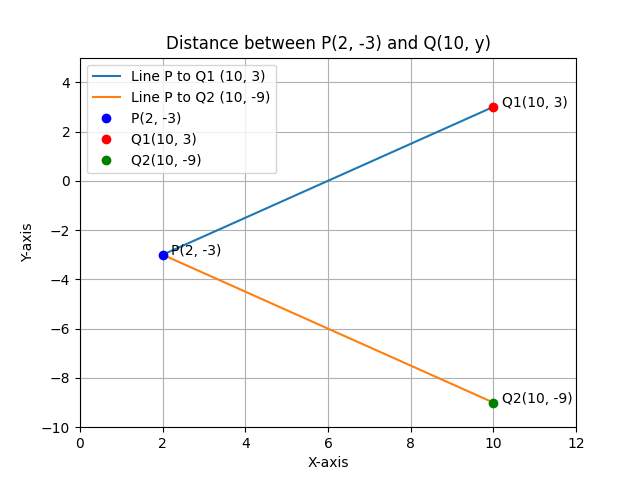
\includegraphics[width=10cm]{figs/figure.png}
    \label{fig:figure}
\end{figure}
\end{enumerate}
\end{document}